%===============================================================================
% $Id: ifacconf.tex 19 2011-10-27 09:32:13Z jpuente $  
% Template for IFAC meeting papers
% Copyright (c) 2007-2008 International Federation of Automatic Control
%===============================================================================
\documentclass{ifacconf}

\usepackage{graphicx}      % include this line if your document contains figures
\usepackage{natbib}        % required for bibliography
\usepackage{subfigure}
\usepackage{enumerate}
%===============================================================================
\begin{document}
\begin{frontmatter}

\title{DORIS - A MOBILE ROBOT FOR INSPECTION AND MONITORING OF
OFFSHORE FACILITIES\thanksref{footnoteinfo}} 
% Title, preferably not more than 10 words.

\thanks[footnoteinfo]{This work is supported primarily by Petrobras S.A. and
Statoil Brazil Oil \& Gas Ltda under contract COPPETEC 0050.0079406.12.9
(ANP-Brazil R \& D Program), and in part by the Brazilian research agencies CNPq
and FAPERJ}

\author[First]{First A. Author} 
\author[Second]{Second B. Author, Jr.} 
\author[Third]{Third C. Author}
\author[Forth]{Forth D. Author}

\address[First]{Research and Development Center, Petrobras/CENPES, Rio de
Janeiro, Brazil} 
\address[Second]{Mathematical Sciences and Technology Department, Norwegian
University of Life Sciences, Oslo, Norwegian }
\address[Third]{Electrical
Engineering Department, COPPE UFRJ, Rio de Janeiro, Brazil, (e-mail: )}
\address[Forth]{TPD RD New Development Solutions, Statoil ASA}

\begin{abstract}                % Abstract of not more than 250 words.
DORIS is a research project which endeavors to design and implement a mobile
robot for remote supervision, diagnosis, and data acquisition on offshore
facilities. The proposed system is composed of a railguided robot capable of
carrying different sensors through the inspected area. This paper presents a
general overview of the robot and a description of the developed embedded
electronics and power supply system. Initial results with teleoperational
navigation validate the concepts considered so far and rise several challenges
for future works.
\end{abstract}

\begin{keyword}
Mobile robots; Field robotics; Decurity and safety of HMS.
\end{keyword}

\end{frontmatter}
%===============================================================================

\section{Introduction}
Safety and efficient operation are imperative factors to offshore production
sites and a main concern to all Oil \& Gas companies. A promising solution to
improve both safety and efficiency is to increase the level of automation on
the platforms by introducing robotic systems.

During the last decade, several Oil \& Gas companies, research groups, and
academic communities have shown an increasing interest in the use of robots for
operation on offshore facilities.  

Recent studies project a substantial decrease in the level of human operation
and an increase in automation on future offshore oil fields
~\cite{skourup2009robotized}.The studies also point out the potential increase
in efficiency and productivity with robot operators, besides the improvement of
Health, Safety, and Environment (HSE) conditions, as robots can replace humans
in tasks performed in unhealthy, hazardous, and confined areas ~\cite{pal}. 
In~\cite{abb}, it is considered the use of robots in Oil \& Gas facilities in
operations that require both high precision and strength, regardless of weather conditions.

In the specific case of Brazil, the Oil \& Gas industry is growing at a high
pace, mainly due to the recent discoveries of big oil fields in the pre-salt
layer off the Brazilian coast. These oil reservoirs are located farther than
300 km from the shore and at depths of 5000 to 7000 km. These factors,
especially the large distances, motivate the development of an offshore
production system with a high degree of automation based on advanced robotics
systems.

Among the research groups interested in offshore robotics, \emph{Fraunhofer
IPA} is pioneer in proposing and demonstrating the applicability of mobile
robots for offshore inspection and maintenance tasks \emph{in
loco} ~\cite{mimroex2}. One example is MIMROex ~\cite{mimroex}, capable of
navigating safely, building maps, and executing inspection tasks autonomously
throughout the topside of platforms.

Another robotic device applied in offshore environments is Sensabot
~\cite{sensabot}, capable of safely inspect and monitor hazardous and remote
production facilities. The robot can sustain high temperatures, is able to
reach areas with difficult access, and is certified to operate in explosive and
toxic environments.

SINTEF-ICT is another group interested in manipulators applied to the oil and
gas industry. Inspection and maintenance operations in a simulated production
process are performed by the cooperation of a gantry-mounted manipulator and a
floor-mounted robot ~\cite{kyrkjebo2009robotic}.

In this paper, we describe the DORIS project, which aims to develop a mobile
robot to perform monitoring, inspection, and simple intervention tasks in an
offshore platform. To this end, the system must be able to move throughout the
monitored environment carrying different sensors, analyzing sensor data
\emph{in loco} or storing it for a posterior analysis, and interpreting the
results. The sensors can identify abnormalities such as intruders in restricted
areas, abandoned objects, smoke, fire, and liquid and gas leakages.
Furthermore, the robot is able to make machinery diagnosis, read instruments,
and perform interventions on valves and other equipment using an embedded manipulator.

The paper is organized as follows: a general overview of the robot and its main
challenges are presented in Section \ref{sec:general_overview}, detailed
descriptions of the embedded electronics, power
supply system and the vehicle support system are taken in
Sections \ref{sec:electronics_overview}, \ref{sec:powersupply_overview}, and
\ref{sec:VSS} respectively.
In Section \ref{sec:results}, preliminary results are shown, and concluding
remarks are drawn in Section \ref{sec:conclusions}. 

\section{General Overview}\label{sec:general_overview}

The proposed system is composed of a robot with cameras, microphones, gas,
vibration and temperature sensors, and a manipulator arm. The robotic device is
guided by a rail and both the robot and the rail follows a modularity concept.
Additional robot modules can be annexed to include other sensors, and the rail
track can be modified by adding or replacing rail segments, thus enabling
operation in different areas of the platform.

The robot will be controlled autonomously or by teleoperation. Task managing
can be either in automatic (programmed using a mission interface) or manual
mode (real-time remote operation). The teleoperation and monitoring
capabilities guarantee online access to the embedded sensors, providing
information about the surrounding environment and the robot operating
conditions with real-time processing. Figure~\ref{fig:DORIS-overview}
illustrates the operation in a production plant.

\begin{figure}[ht] 
\centering
\subfigure[Robot's operational scenario in a production plant]{%
    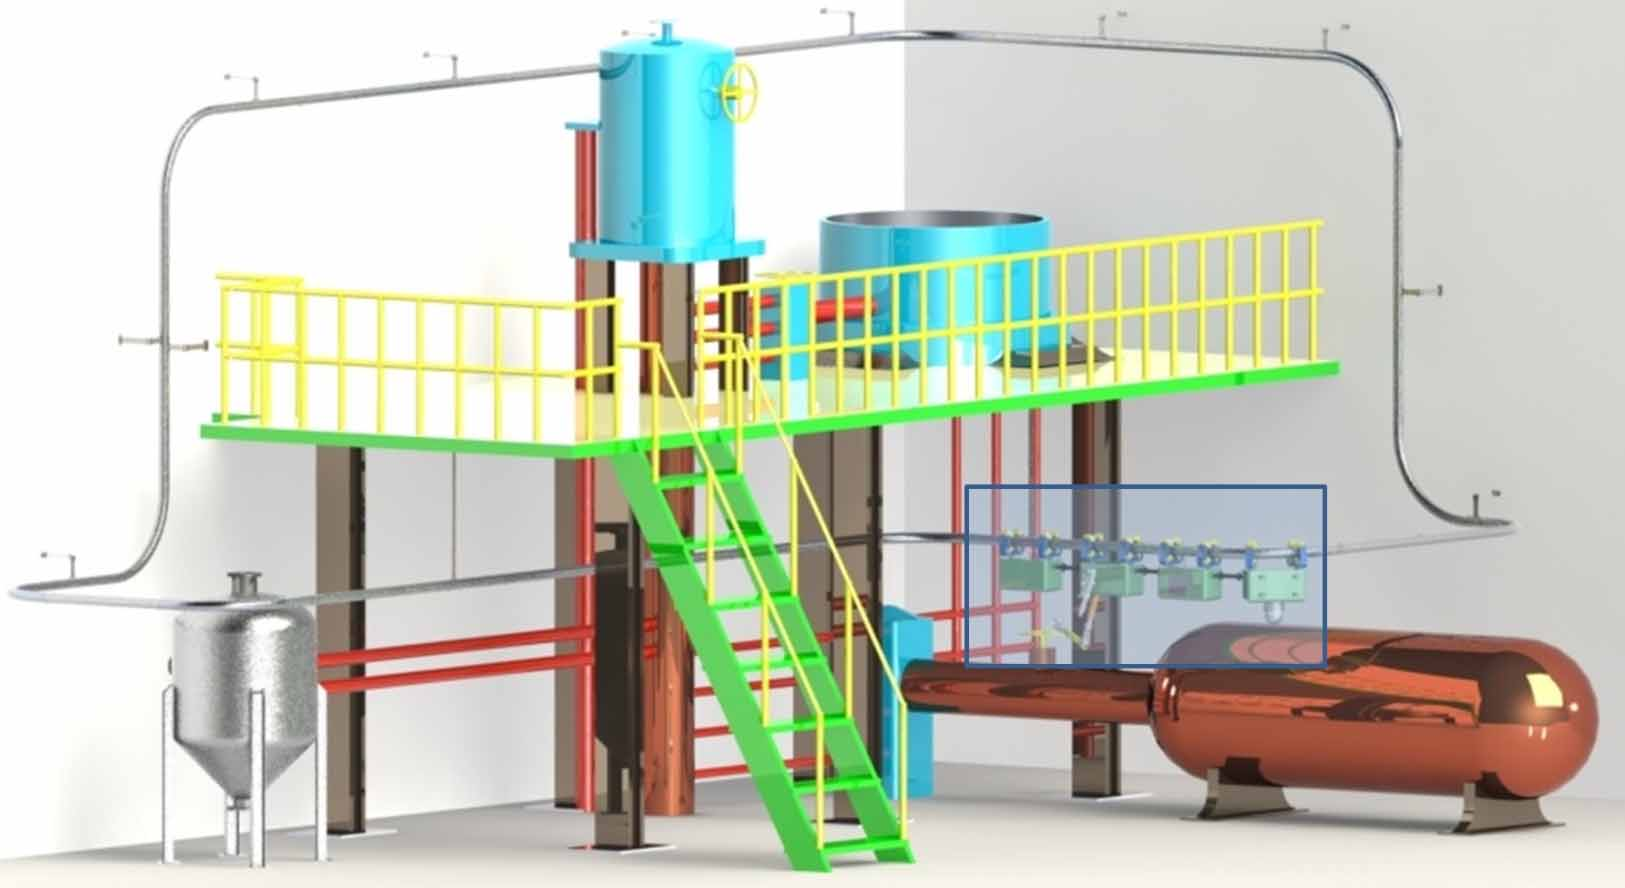
\includegraphics[width=8.4cm]{figs/cenario1.jpg}  % width is 7.6 cm.
    \label{fig:cenario1}} 
\subfigure[Detailed zoom of the robot]{%
    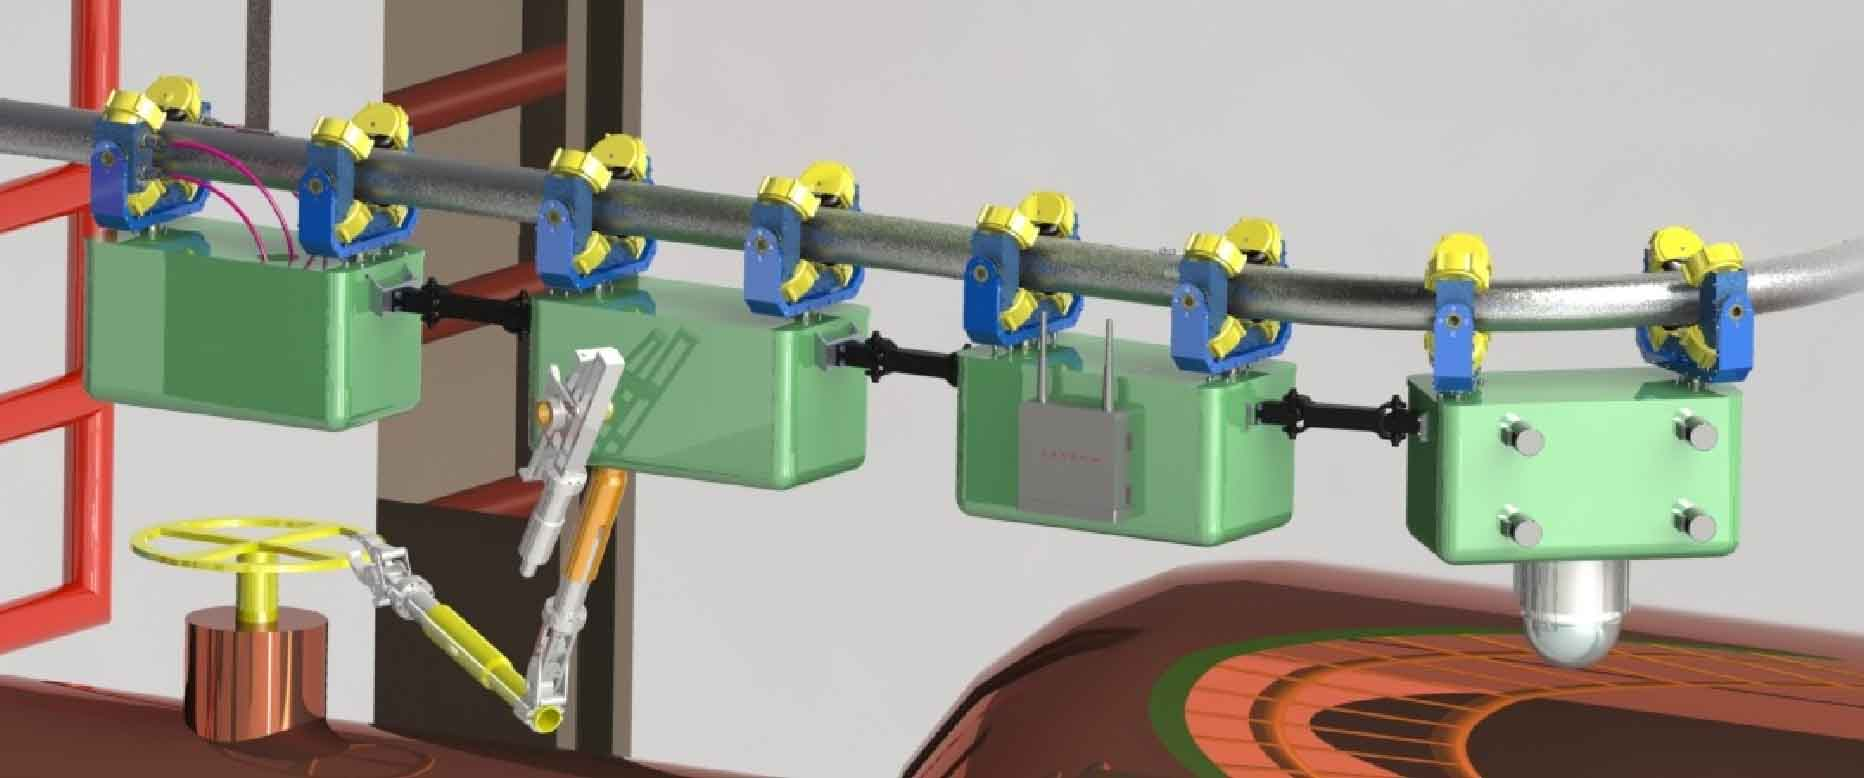
\includegraphics[width=8.4cm]{figs/zoom.jpg}  % width is 7.6 cm.
    \label{fig:zoom}}\vspace{-.1cm}
\caption{Illustration of the DORIS robot operating in a production plant.}\vspace{-0.25cm}
\label{fig:DORIS-overview}
\end{figure}

The DORIS project can be divided into five subsystems: electronics, power
supply, software, mechanics and signal processing.

%-------------------------------------------------------------------------------------------------------------------------
%ELECTRONICS
%-------------------------------------------------------------------------------------------------------------------------
The electronics subsystem is responsible for providing embedded computational
support for the robot control, signal processing, task managing, and local and
remote communication. The device motion is controlled through drivers that can
receive position, velocity, or current setpoints. The embedded electronics has
two printed circuit boards for the vehicle support system: energy distribution
and monitoring, basic failure detection, emergency handling and devices'
control.

%-------------------------------------------------------------------------------------------------------------------------
%POWER SUPPLY
%-------------------------------------------------------------------------------------------------------------------------
The power supply system uses military-class lithium-ion batteries, which have
small size and high energy capacity. In the first prototype of DORIS, four
batteries are used to power the motors and two to power the other electronics
components. 


%-------------------------------------------------------------------------------------------------------------------------
%SOFTWARE
%-------------------------------------------------------------------------------------------------------------------------
The main objective of the software subsystem is to allow the implementation of
high- and low-level control of the robot. The tools used to develop DORIS
software architecture must consider two important factors: they have to be
commercially available, and provide modular functionalities. These requirements
led to the adoption of Qt as the graphical interface framework ~\cite{qt},
Robot Operating System (ROS) as the communication middleware ~\cite{ros}, and
Ubuntu as the operating system.

The software provides autonomous control (programmed tasks) and remote control
through a Graphical User Interface (GUI) in the Host Control Base (HCB)
computer. The HCB is composed of a set of processes running in parallel
denominated ROS nodes, which can communicate with each other. To deal with this
environment, a new software architecture called Robot Package Software is
proposed, dividing the software into tools (graphical windows) and components
(processing and communication unities), and grouping them into a dynamic
library. 

%-------------------------------------------------------------------------------------------------------------------------
%Mechanics
%-------------------------------------------------------------------------------------------------------------------------
The mechanical project designs the rail, the
traction and passive modules, and the joints used to couple them. The design
allows the robot to move smoothly in a 3D space and makes full stop anywhere
on the rail. Considering the severe corrosion and weather conditions in
offshore environments, the choice of materials are imperative to the success of
the project and certified solutions must be considered.

The robot is composed of two modules at its default configuration, but it is
conceived so that other modules can be added. The total weight of this
configuration is estimated at 50 kg and we expect to have a maximum speed of
1m/s.

The design incorporates the use of gimbals with wheels as guides for
the module on the rail \cite{cba}. In the new configuration, the motors are
fixed on the gimbal and transmit its torque to the wheels via spur gears. The use of gimbals
is an proper choice concerning stability, guidance, and support. Furthermore,
it is possible to have a smooth vertical motion applying radial forces by the
clamping mechanism.

%-------------------------------------------------------------------------------------------------------------------------
%DSP
%-------------------------------------------------------------------------------------------------------------------------
The signal processing capabilities of the robot are \cite{cba}: (a) Video: use
of multiple cameras (visible-light, infrared, fisheye and stereo) to detect
video anomalies such as abandoned objects, smoke, fire, liquid leakage, and
intruders. (b) Audio: detection of audio anomalies of impulsive nature, such as
an explosion or the diagnosis of rotating machines based on energy and pitch
(fundamental frequency) signatures using a single or a array of microphones. (c)
Vibration analysis: Use of acceleration sensors to diagnose the operation mode
of rotating machines, performing possible fault classification, such as
 misalignment and unbalancing operation. (d) Gas sensor: detection of gas
 leakages. (e) 3D mapping: environment 3D modeling using a laser sensor.

The main idea of all these signal processing features is to make the robot
perform an initial reference lap around the closed rail track, being manually
validated by a system operator. In the subsequent laps, all signal processing
algorithms compare the newly acquired signals with the reference data to detect
any form of anomaly, as indicated above. Once an anomalous behavior is
detected, an alarm is flagged to the system, which stores all associated data
for immediate or future diagnosis.


%-------------------------------------------------------------------------------------------------------------------------
%OTHER CHALLENGES
%-------------------------------------------------------------------------------------------------------------------------
Considering the robot functionalities and the aggressive offshore environment,
several challenges should be addressed. Temperatures in offshore facilities can
vary between $-30^{\circ}$C to $50^{\circ}$C, relative humidity can reach
100\%, and there may be splash water, salty air, storms, and high extensive
corrosion ~\cite{graf2007mobile}. 

Concerning robustness and safety required to operate in classified areas, the
robot must be sealed against water and objects, resistant to a wide temperature
range, protected from impact and vibration, electrically shielded to avoid
explosion by ignition, and equipped with a monitoring system.


Another challenge is that the embedded computers must run heavy signal
processing algorithms, requiring high computational power. However, the power
supply subsystem must efficiently provide power and maintain a low level of
power consumption.

Further complications arise because the system is designed to move in confined
areas and have efficient wireless communication with operators, providing
online information of sensors data. Finally, the robot must have a modular and
flexible design, employing plug and play extensions.


\section{Embedded Electonics}\label{sec:electronics_overview}
The embedded electronics (EE) is composed of the following subsystems:
communication system, actuator control system, vehicle support system, and
sensor integration system. 

The communication system is composed by \emph{Local Area Network (LAN)} and
2.4/5.0 GHz radio. 
\newline
The LAN is a Gigabit Ethernet network inside DORIS and Wi-Fi IEEE
802.11n as the main communication between DORIS and the remote control base.
DORIS can be remotely operated from an remote control base located at the
offshore facility. Wi-Fi communication is used for normal mode, and 2.4/5.0 GHz
radio communication is used for emergency mode.

Inside the robot, the Ethernet network connects DORIS main devices: computer,
three cameras, Wi-Fi access point and PCBs. These are managed by a Gigabit
Ethernet Switch. The Wi-Fi communication between DORIS and base is achieved
using one Wi-Fi access point at the robot and one at the base. This LAN
topology allows, with room to spare, the fast communication of video and images
from all main cameras, which is needed by the computer for a video and
audio real-time processing and transmitting. In addition, the use of an Ethernet
Switch allows the easy expansion of the Ethernet network for additional modules.

Other peripheral devices may need USB communication, which is available at the
computer ports. An overall scheme of the EE system is shown at
figure~\ref{fig:EE-Communications}.
\begin{figure}
\begin{center}
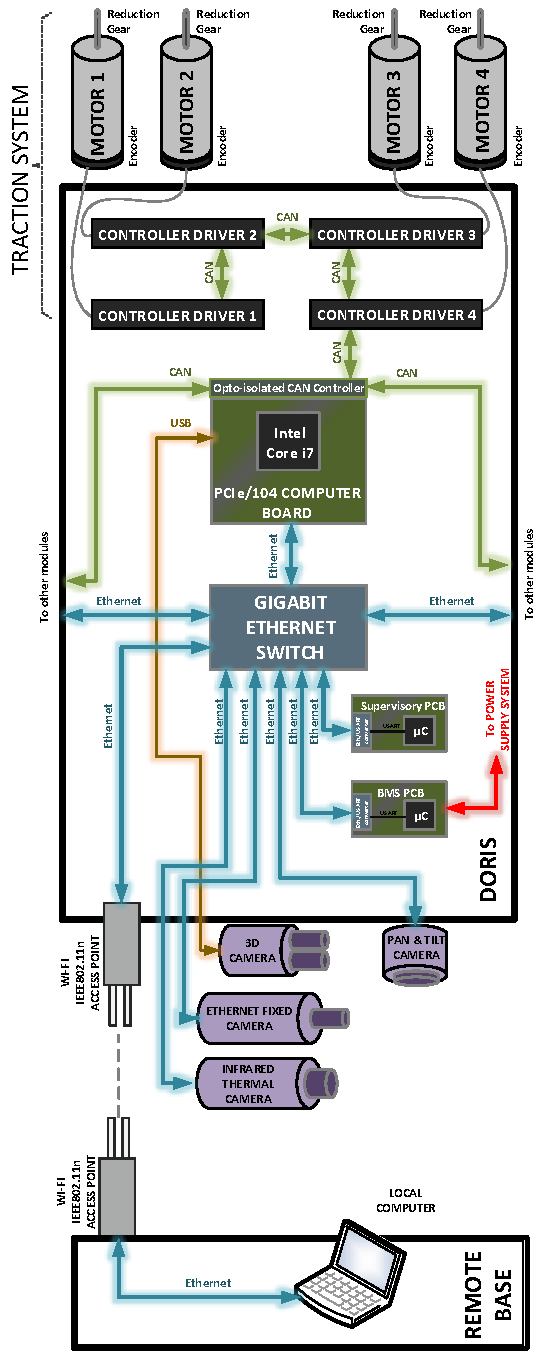
\includegraphics[width=8.4cm]{figs/EE-Communications.pdf}    % The printed column width is 8.4 cm.
\caption{Embedded Electronics system: overall scheme}
\label{fig:EE-Communications}
\end{center}
\end{figure}

The actuator control system is composed by the CAN network for DORIS
traction, 4 motor packs containing 1x EC brushless motor, 1x encoder and 1x
21:1 reduction gear, 4 controller drivers and respective cable/connector set.
The computer, which is the DORIS main decision/action center, communicates with
the drivers via CAN, since it is suitable for a real-time control and provides
a strict error control for message transmission. Since the traction system
generates a significant amount of conductive noise, a galvanic opto-isolator is
used between the CAN and the computer to minimize interference on the rest of
the EE system.

The \emph{Vehicle Support System (VSS)} composed by microcontroller based
\emph{printed circuit boards (PCBs)} for: failure detection; device protection;
energy distribution and monitoring; emergency handling\cite{MARIUS}. The VSS
functionalities is detailed in section\ref{sec:VSS}. 

The sensor integration system is composed by all DORIS sensors and the interface
between devices and the computer. The subsystem enables inclusion,
reconfiguration and replacement of peripheral device. The sensor data
integration is carried out by an high performance Intel\textregistered
Core\texttrademark i7 computer embedded in a PCIe/104 form factor board.
  
\section{Power supply system}\label{sec:powersupply_overview}
This part of the robot is responsible for reliable, safe and efficient delivery
of electric energy on each equipment inside DORIS. The power supply is a high
density energy level military lithium ion battery model, which comes with
intrinsically safety circuit in order to avoid possible short-circuits or heat
problem, disabling the battery itself in cases of safety risks. The model
currently in use has a 10Ah capacity, where four units are located on each
module, weighting 1.4Kg each.

As Verma et al. (2004) highlights, robots often operate in environments where
human intervention is expensive, slow, unreliable, or impossible. It is
therefore essential to monitor their behavior so that faults may be addressed
before they result in catastrophic failures. The power management interface is
implemented through System Management Bus (SMBus) connections with the robot
microprocessor, allowing the electronics to receive all possible information
about each battery condition, see \ref{sec:VSS}. 

In order to avoid avoid EMI and conductive noise interference, the project
currently works with two separate power buses, each of these built using two
24Vdc batteries connected in parallel, being able to deliver a capacity of
20Ah. One bus is dedicated to power the motors and the other to power all
electronic devices. Also, DC/DC converters are
being used to create different voltage levels (12Vdc and 5Vdc) and to
ensure a stable power source (even for 24Vdc components). 

Seeking power protection, Diodes are being used in order to avoid back-flow
current, fuses are protecting the system from undesired peaks just after each
DC/DC converter and buttons allow power buses to be separately turned on/off.


The current architecture of the power supply embedded on this project is
illustrated on figure~\ref{fig:DiagramaSAM}. The electronics' power bus uses
14AWG wires for up to 15A of nominal current and the motors' uses
12AWG wires for up to 21A of nominal current.

\begin{figure}[ht]
\centering
%\subfigure[Robot's operational scenario in a production plant]{%
    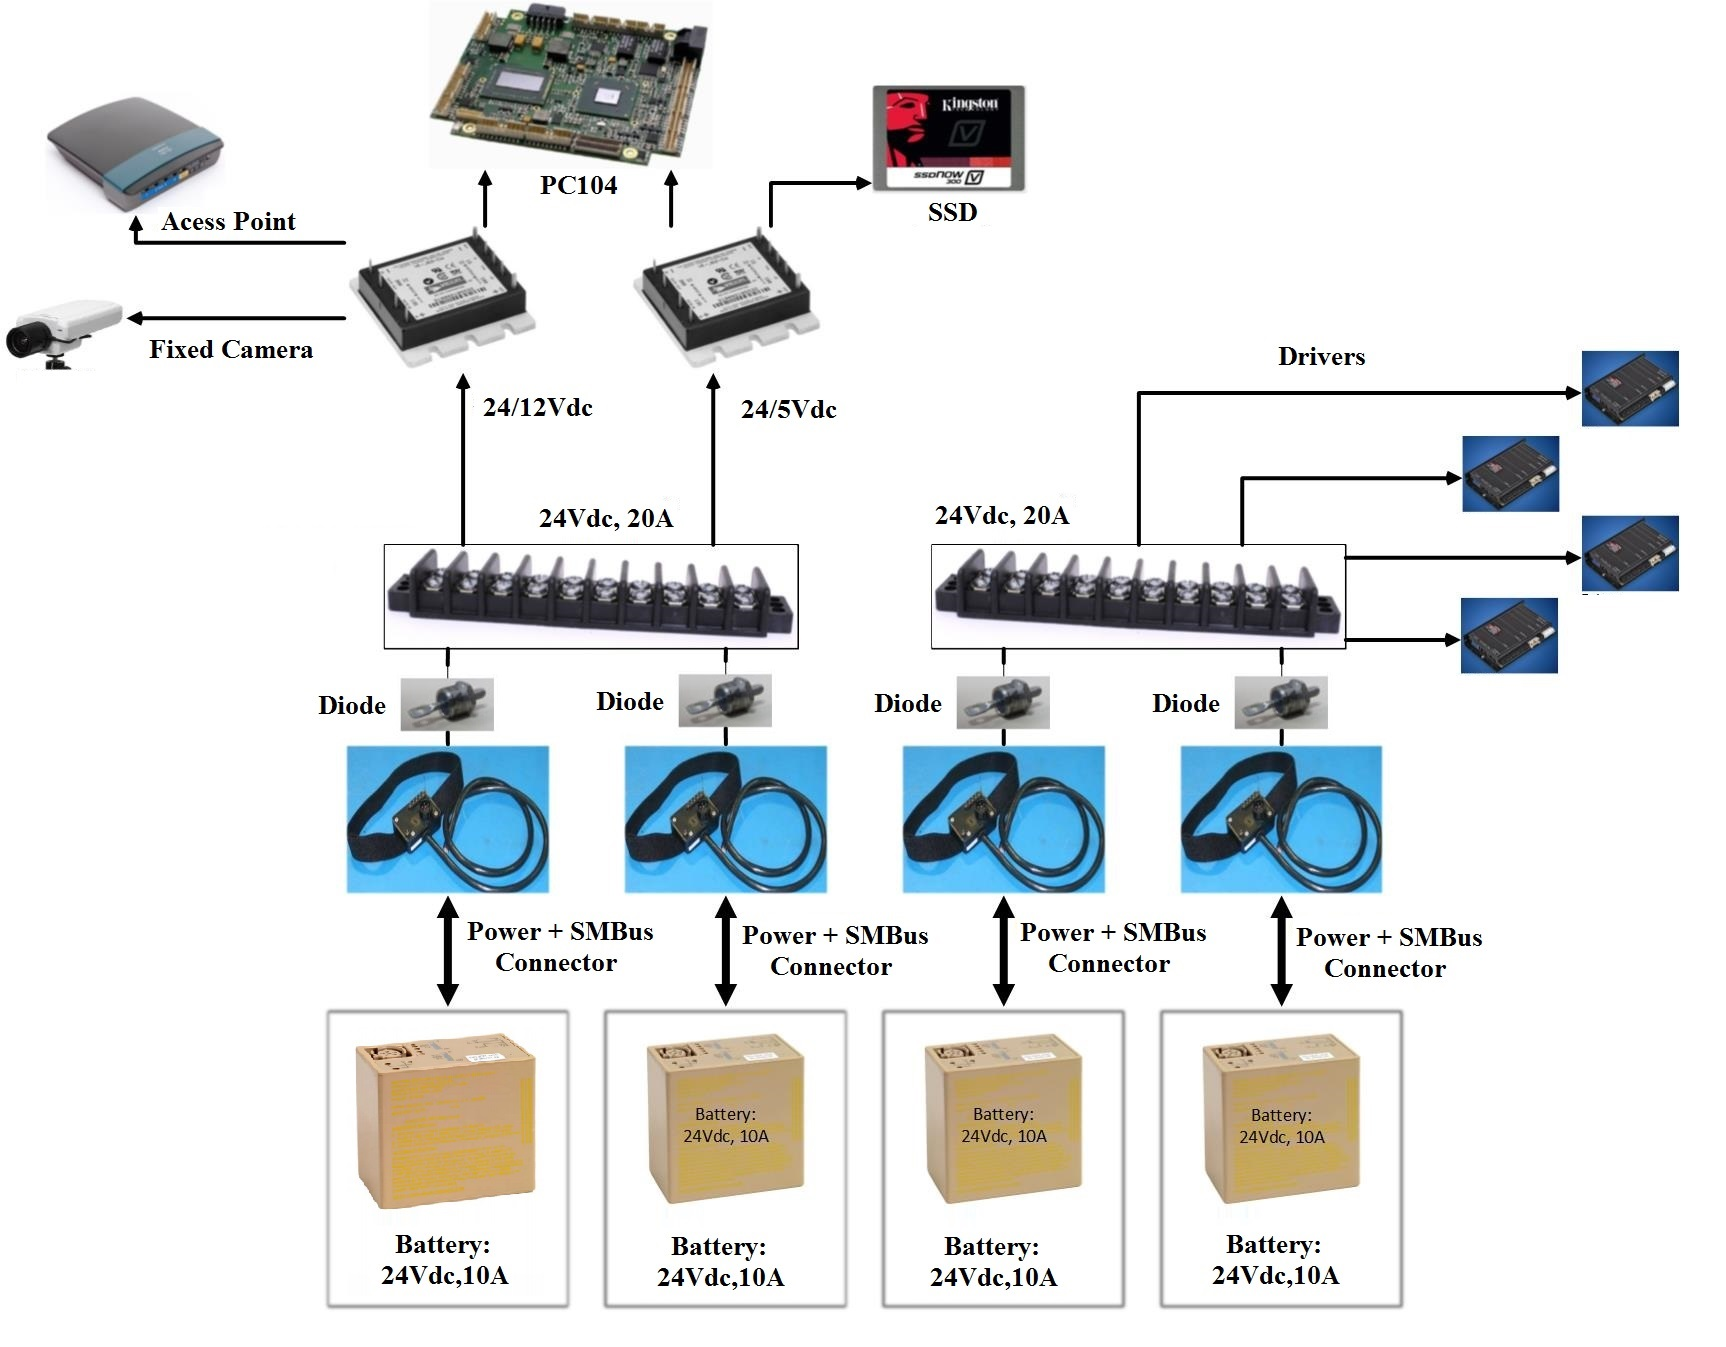
\includegraphics[angle=90,width=1\columnwidth]{figs/DiagramaSAM.jpg}  % width is 7.6 cm.
    \label{fig:DiagramaSAM}
\caption{Power Supply Architecture.}\vspace{-0.25cm}
%\label{fig:DORIS-overview}
\end{figure}

Considering this, new challenges came up in order to improve the features of
the system.

\section{Vehicle Support System}\label{sec:VSS}

As one of the main contribution of this article, DORIS is equipped with a
\emph{Vehicle Support System (VSS)} composed by microcontroller based
\emph{printed circuit boards (PCBs)} for: failure detection; device protection;
energy distribution and monitoring; emergency handling. The VSS functionalities
are:
  
\begin{itemize}
    \item Failure detection is achieved by the monitoring of devices'
    current/voltage and module humidity/temperature.
    \item Peripheral devices are protected against overcurrent by fuses and
    solid-state relays, which can be turned on/off at any time automatically
    upon a detected failure or manually via operator.
    \item Energy distribution and monitoring is achieved by the \emph{Battery
    Management System (BMS)}. Each battery pack is monitored via SMBUS
    communication, which allows the reading of the battery status, voltage,
    current, temperature and remaining charge, besides other variables. This
    information allows the PCB embedded microcontrollers to provide adequate
    power balance in extreme situations (e.g.: demand of full power to either
    traction system or electronics system) or reconfiguration of power supply
    distribution in case of failures. 
    \item In emergency cases, the robot can be turn on/off using a physical
    \emph{emergency shutdown (ESD)} button or via radio. The radio system can
    also replace Wi-Fi in some functionalities if it fails.
  \end{itemize}
  
DORIS VSS includes three board types: i) supervisory system
%(figure~\ref{fig:SSPCB})
; ii) Battery Management System - BMS
%(figure~\ref{fig:BMSPCB})
; iii) BMS Switching board%~\ref{fig:BMSSB}.

The supervisory board is composed by: two AVR micrcontrollers, solid-state
relays (max. 1.5A), hall effect sensors (HES - for current measurements),
16-channels analog-to-digital converter (ADC), humidity/temperature (T/H)
sensor, and an Ethernet-to-UART converter. 

Four supply channels, 5, 12, 24 VDC from the DC-DC converters boards, are
connected to solid-state relays, these to a hall-effect sensor and the last to
the ADC. The T/H sensor provides the module internal humidity and temperature,
and sends the information to the AVR. The AVR interprets ADC's and T/H's data,
then sends the results to the Ethernet module. These information corresponds to
the monitoring data. 

Besides the monitoring, AVR can protect devices against overcurrent by
commanding the open/close of the relays. It can be also done manually by the
operator. Thus, the AVR accumulates the role of: managing the collected
data, transmit data to computers, react to computer commands and react to
faulty situations.
 
The BMS composition is similar to the supervisory system, with the following
differences: no solid-state relays for device on/off; no hall-effect sensors;
communication with batteries via \emph{SMBUS (System Management Bus)};
connection with the BMS bus switching board. The SMBUS is used to get important
information from the batteries, such as: temperature, voltages, currents and
remaining charge. 

The BMS bus switching system contains high power solid-state relays (20A). They
can be commanded from the BMS AVR in order to adequate distribute the power to
either motor bus or electronics bus. The AVR decisions about the better
distribution is based primarily on data collected via SMBUS.

% \begin{figure}
% \begin{center}
% 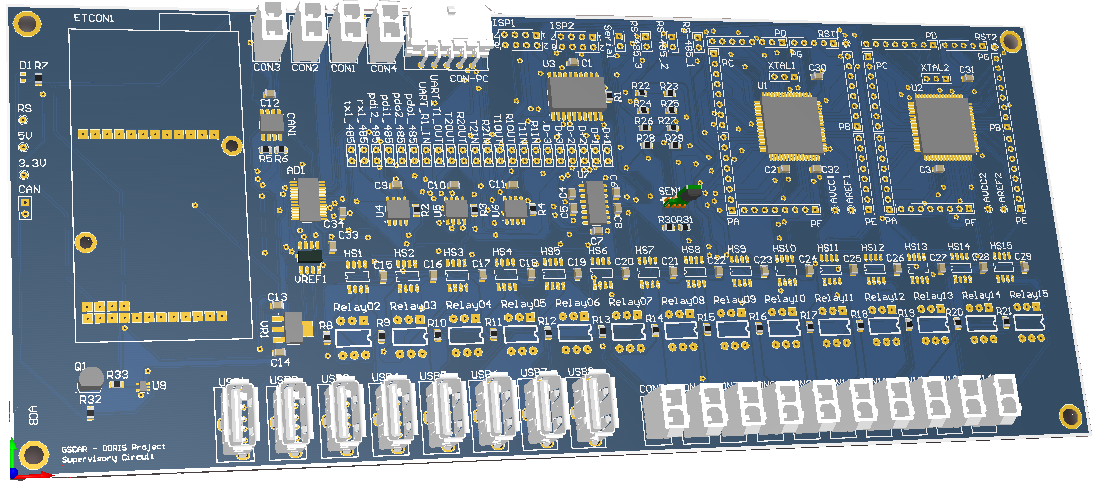
\includegraphics[width=8.4cm]{figs/SSPCB.png}    % The printed column width is 8.4 cm.
% \caption{Supervisory system PCB: 3D illustration}
% \label{fig:SSPCB}
% \end{center}
% \end{figure}
% \begin{figure}
% \begin{center}
% 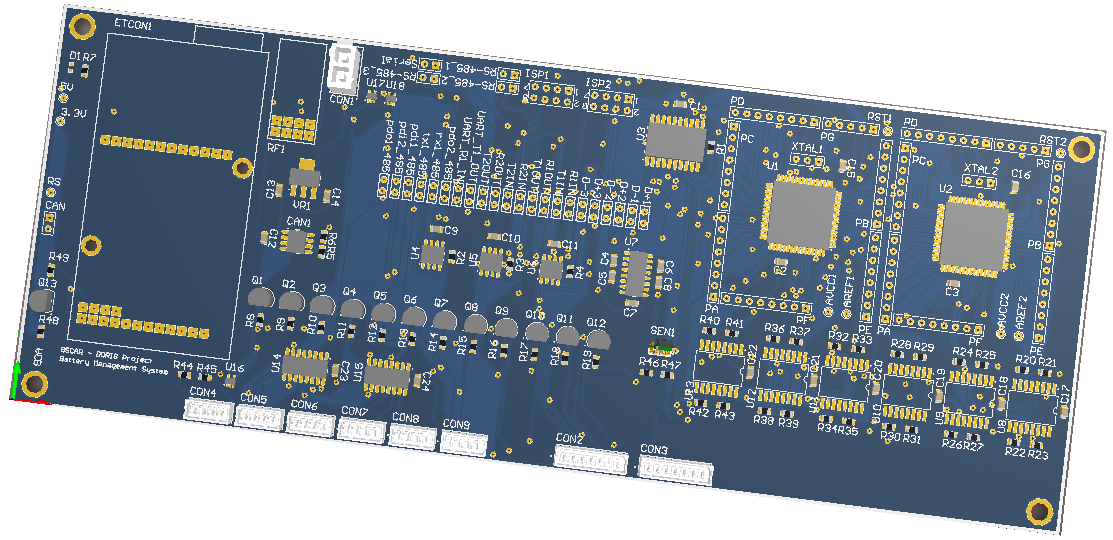
\includegraphics[width=8.4cm]{figs/BMSPCB.png}    % The printed column width is 8.4 cm.
% \caption{Battery Management System PCB: 3D illustration}
% \label{fig:BMSPCB}
% \end{center}
% \end{figure}
% \begin{figure}
% \begin{center}
% 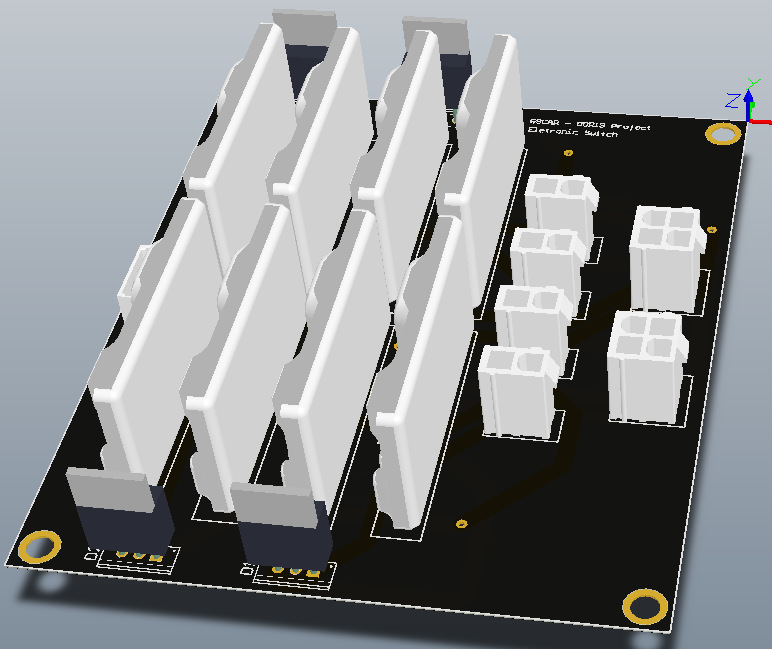
\includegraphics[width=8.4cm]{figs/Top2.png}    % The printed column width is 8.4 cm.
% \caption{Illustration of the Power Bus Switching Boards Options.}
% \label{fig:BMSSB}
% \end{center}
% \end{figure}

\section{Results}\label{sec:results}
A DORIS prototype, Single Autonomous Module (SAM), was built
with low cost materials for tests of all concepts above. And specific tests of
the VSS was implemented outside the vehicle. The two subsections below detail
the tests.

\subsection{Single Autonomous Module (SAM)}

The DORIS prototype, SAM (single autonomous module), was built
with low cost materials and was tested in horizontal and vertical motion on a
rail composed of straight and curved modules. A tubular track built using
straight and curved segments was installed in the GSCAR laboratory, in
COPPE/UFRJ. The track comprises all possible movements that the robot must
make.

The first objectives of (Fig.~\ref{fig:SAM2}) is to test the following concepts:
\begin{itemize}
  \item Mechanical: the use of gimbals for guidance, stability, and weight
  support; The traction system;
  \item Power supply: independent buses for motors and electronics devices;
  batteries robustness and duration;
  \item Electronics: sensor integration; communication system;
  \item Software: teleoperation; user interface;
  \item Digital processing: video streaming;
  \end{itemize} 

% \begin{figure}[!h]
% \begin{center}
% 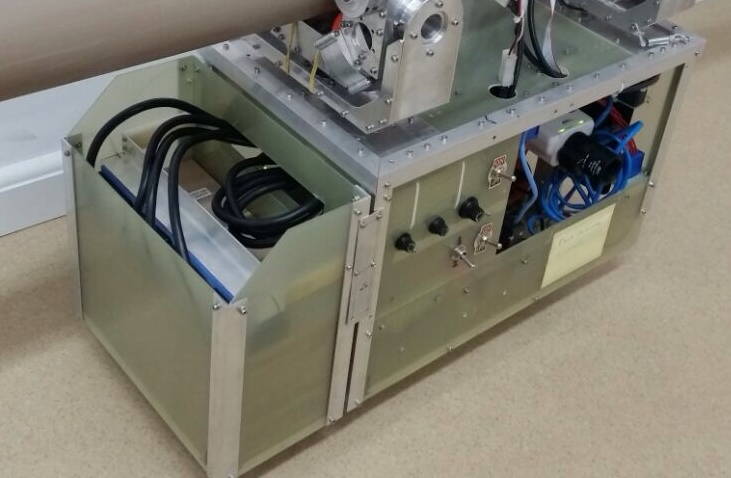
\includegraphics[width=8.4cm]{figs/SAM1.jpg}  % width is 7.6 cm.
% \label{fig:SAM}
% \caption{Single Autonomous Module}
% \end{center}
% \end{figure}
\begin{figure}[!h]
\begin{center}
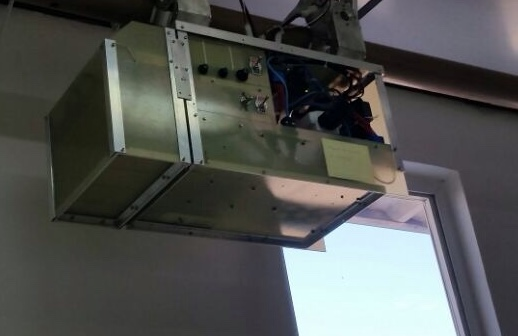
\includegraphics[width=8.4cm]{figs/SAM2.jpg}  % width is 7.6 cm.
\label{fig:SAM2}
\caption{Single Autonomous Module}
\end{center}
\end{figure}

%-------------------------------------------------------------------------------------------------------------------------
%TESTES/RESULTADOS
%-------------------------------------------------------------------------------------------------------------------------
Initial tests performed with the prototype show good performance of the gimbals
in terms of stability. Even though the gimbals may shake slightly due to
irregularities on the rail surface and asymmetrical positioning of the guide
wheels, the base keeps a steady orientation while moving.

The independent buses works efficiently, and batteries were able to supply
energy for all system. An issue observed on this project
is the fact that when going downwards the motor generates energy. Depending on
the height of the fall and the velocity of DORIS, the energy created may reach
voltage levels that cause the drivers to stop.

All SAM's devices: ethernet fixed camera, 3D webcam, wireless router, drivers,
and embedded computer with SSD, were integrated with the system and communicates
as expected. 

SAM can be teleoperate from Statoil to GSCAR lab, in Rio de Janeiro, Brazil,
with the user interface developed in Qt environment.

\subsection{Vehicle Support System Tests}
%Finally, the traction system mounted on a prismatic mechanism did not work properly. The prismatic joints locked in certain circumstances and the weight of the traction system led to loss of contact between the lower part of the grooved wheels and the tube. This results suggest investigating an alternative concept for the traction system, for example moving the traction to the gimbals wheels, as presented in Section \ref{sec:mechanics_overview}. 
\section{Conclusion and Future work}\label{sec:conclusions}

In this paper, we presented the DORIS project, which endeavors to develop an
offshore facilities inspection and monitoring robot. The prototype is based on
rail guided modules powered by a battery system and equipped with multiple
sensors that enable detection of anomalies, such as abandoned objects and gas
leakage. 

A prototype, SAM, was built to test mechanics, electronics, power
supply, software architecture, and digital processing concepts.
Preliminary results show good overall performance of: the guidance system using
gimbals; sensor integration and communication; independent power buses for
electronics and motors; teleoperation; and video streaming.

%Thus, DORIS is equipped with a power supply system with an improved robustness
%level when compared with other robotic systems and it also has a considerable
%light weight, high energy density and increased safety properties.

The Vehicle Support System was tested outside the robot and the customized
printed circuit boards were able to monitor: the batteries via SMBUS,
temperature/humidity, DC/DC voltage levels, and devices's currents. The
solid-state relays can also turn on/off the devices for protection and/or
efficiently power consumption.

The future challenges are related to the expansion of DORIS functionalities,
as described below:
\begin{enumerate}[i)]
  \item \emph{Expansion and reconfiguration of robot modules}:\\
  \newline
  DORIS will need more than one module to support more devices and features.
  The EE system permits the free expansion and reconfiguration of DORIS
  modules, achieved by the introduction of a bus topology for DORIS
  main networks: Ethernet and CAN. However, the junction between wagons is a
  mechanical challenge and is the next step for the mechanics' group.\\
  \item \emph{Autonomous operation}:\\
  \newline
  DORIS autonomous operation is a challenge for the software development. The
  Positioning System, comprising wheels' encoder (odometry) and
  fixed camera (3D mapping), will be upgraded with an inertial movement unit
  (IMU) and a laser scanner. The sensor's fusion will precise the Navigation
  System, which estimates the linear position and velocity of the vehicle. Also,
  a Mission Control System need to be developed for the operator.
  \\
  \item \emph{Manipulator control}:\\
  \newline
  It is planned the inclusion of a robotic manipulator fixed at the module
  bottom. It is going to handle a vibration sensor and a 3D camera at the grip.
  Besides the prismatic movement of the robot along the rail, the manipulator
  may need more 4 degrees of freedom, excluding the \emph{roll orientation}.
  Since it is actuated by electric motors just like the traction system, it
  will be controlled via CAN bus.\\
  \item \emph{Reduced interferences, such as Electromagnetic interference (EMI) and electrostatic charge}:\\
  \newline
  Future DORIS improvements should include a well designed/installation of the
  shield network and earthing system to reduce EMI. An electrostatic discharger
  should be designed to drain the accumulated charge from the shielding system.
  \item \emph{DORIS's downward motion}
  \newline
  An issue observed on power supply system is the fact that when going downwards
  the motor generates energy. Depending on the height of the fall and the velocity
  of DORIS, the energy created may reach voltage levels that cause the drivers
  to stop. Because of this, the group is working on ways to measure de energy
  level created and decide if it would be worth to store this energy or if it
  would be better to simply discard it by using a shunt regulator.
  \item \emph{Motors' noises}
  \newline
  The digital processing is working on an audio filter for the DORIS motors,
  which generates a lot of noise when working at higher speeds.
\end{enumerate}

\bibliography{ifacconf}             

\appendix
 
\end{document}
